\subsection{Gate dell'ADC}

Variamo la durata del gate dell'ADC e calcoliamo il rapporto $\sigma\!/$\!media per il picco di annichilazione rivelato dal PMT1, modellato come al solito con una gaussiana.
\marginpar{Aggiungere una locuzione o frase introduttiva.}
Su alcune misure abbiamo introdotto dei ritardi per migliorare o peggiorare la sincronizzazione con il gate al fine di quantificare quanto la messa in tempo influisca sulla nostra risoluzione. Il risultato di questa misura è in \autoref{fig:gate}, i dati sono in \autoref{tab:gate}.
\marginpar{Dove sono finiti i ritardi nella tabella?}

\begin{figure}[h]
\centering
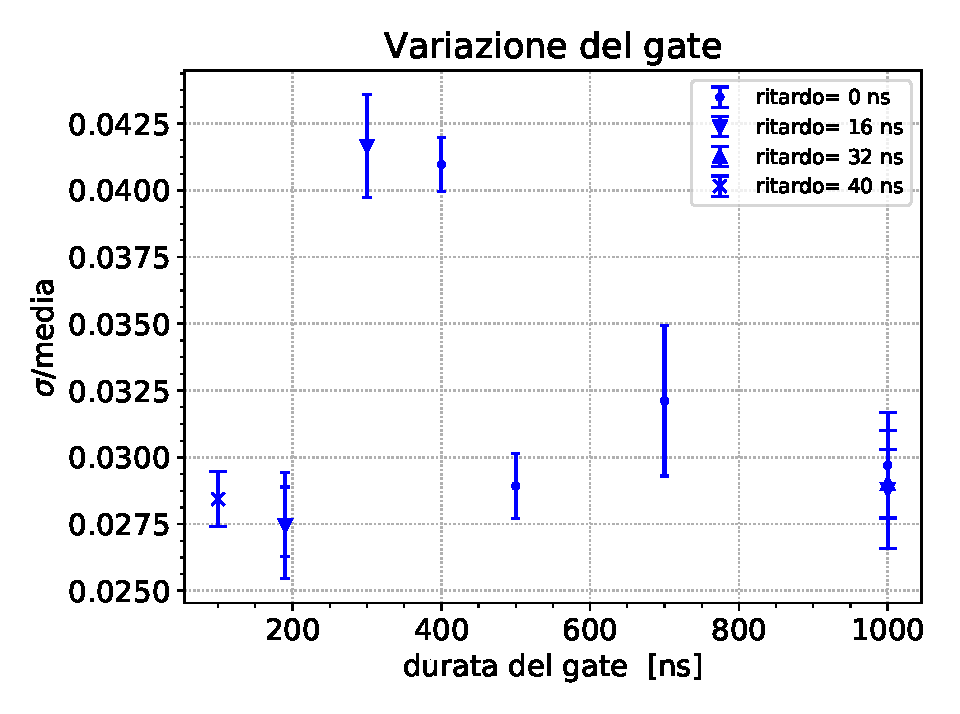
\includegraphics[width=20 em]{immagini/gate}
\caption{Grafico della risoluzione in funzione della durata del gate. Le misure sovrapposte sono state ottenute ritardando il segnale del PMT1.}
\label{fig:gate}
\end{figure}

\begin{table}[h]
\centering
\begin{tabular}{c|c|c|c}
durata (ritardo) [ns] & media [digit] & $\sigma$ [digit] & $\sigma\!/$\!media\\
\hline
 100 & 304.88$\,\pm\,$34 &  8.67$\,\pm\,$31 & 0.0284 $\,\pm\,$10 \\  
 190 & 492.82$\,\pm\,$50 & 13.59$\,\pm\,$65 & 0.0276 $\,\pm\,$13 \\
 190 & 513.05$\,\pm\,$80 & 14.1 $\,\pm\,$1.0 & 0.0274$\,\pm\,$20 \\
 300 & 307.68$\,\pm\,$36 & 12.81$\,\pm\,$59 & 0.0416 $\,\pm\,$19 \\
 400 & 344.25$\,\pm\,$25 & 14.10$\,\pm\,$34 & 0.0410 $\,\pm\,$10 \\
 500 & 524.01$\,\pm\,$42 & 15.16$\,\pm\,$64 & 0.0289 $\,\pm\,$12 \\
 700 & 482.54$\,\pm\,$85 & 15.5 $\,\pm\,$1.4 & 0.0321$\,\pm\,$28 \\
1000 & 539.43$\,\pm\,$61 & 16.0 $\,\pm\,$1.1 & 0.0297$\,\pm\,$20 \\
1000 & 553.88$\,\pm\,$71 & 15.9 $\,\pm\,$1.2 & 0.0288$\,\pm\,$22 \\
1000 & 542.68$\,\pm\,$41 & 15.75$\,\pm\,$69 & 0.0290 $\,\pm\,$13 
\end{tabular}

\caption{Andamento della risoluzione in funzione della durata del gate. I numeri tra parentesi indicano di quanto è stato ritardato il PMT1.}
\label{tab:gate}
\end{table}

Dall'analisi dei dati abbiamo potuto vedere che, fatta eccezione per le misure a \SI{300}{ns} e \SI{400}{ns}, la risoluzione dell'ADC è compatibilmente la stessa.
Abbiamo allora deciso di porre la durata del gate a \SI{550}{ns} perché era il valore usato prima di questa misura.
Questa scelta è poi diventata \SI{1}{\micro s} nell'apparato B per evitare problemi derivanti dal jitter dei segnali. Infine notiamo che cambiare i ritardi sui segnali in ingresso non influisce significativamente sulla risoluzione dell'apparato.
\marginpar{Ma li abbiamo cambiati di pochissimo rispetto ai tempi in gioco,
quindi non vale dire che non influiscono significativamente.}